%
% IT.
% Information Technology
%
% Aleph Objects Operations Manual
%
% Copyright (C) 2014, 2015 Aleph Objects, Inc.
%
% This document is licensed under the Creative Commons Attribution 4.0
% International Public License (CC BY-SA 4.0) by Aleph Objects, Inc.
%

\section{Servers}
In general, the servers are all running the latest stable release of Debian,
Jessie, version 8, on the amd64 architecture. Some are running Wheezy because
the daemon they hosts prefers it. There is some Debian Squeeze, which is being
migrated. The firewalls are OpenBSD. There is one CentOS and one Fedora
machine.

All machines are backed up at least daily. Updates are run at least weekly,
sooner depending on the nature of the update.

\subsection{Aleph Mountain Servers}
This is a list of servers and nodes that are in the Aleph Mountain building.

\begin{itemize}
\item \texttt{abejas.alephobjects.com} --- Apache, OpenERP.
\item \texttt{amfw1.alephobjects.com} --- OpenBSD, PF.
\item \texttt{amfw2.alephobjects.com} --- OpenBSD, PF.
\item \texttt{aobuild1.alephobjects.com} --- Compile/build server.
\item \texttt{aocluster1.alephobjects.com} --- 3D Printer cluster Botqueue
       server.
\item \texttt{aodb.alephobjects.com} --- Postgres.
\item \texttt{aogfs1.alephobjects.com} --- Test, potential fileserver.
\item \texttt{aomds1.alephobjects.com} --- Test, potential db server.
\item \texttt{cam.alephobjects.com} --- Motion, Motioneye video camera server.
\item \texttt{jebstation.alephobjects.com} --- sshfs file server.
\item \texttt{tunk.alephobjects.com} --- apt-cacher, OpenVPN server, dnsmasq
      (dhcp, dns cache, tftp), MySQL, OpenLDAP.
\end{itemize}

\subsection{Virtual Servers Elastichosts Los Angeles}
These are machines ``in the cloud''.

\begin{itemize}
\item \texttt{aomail.alephobjects.com} --- Apache, Roundcube.
\item \texttt{analytics.alephobjects.com}  --- Apache, Piwik, MySQL.
\item \texttt{cal.alephobjects.com} --- Calendarserver.
\item \texttt{develdrupal.lulzbot.com} --- Test server. Apache, Drupal,
       Ubercart, MySQL.
\item \texttt{develerp.alephobjects.com} --- Test server. OpenERP, Postgres.
\item \texttt{dodev.alephobjects.com} --- Test server. Odoo, Postgres.
\item \texttt{drupalsql.lulzbot.com} --- MySQL.
\item \texttt{drupalsqlslave.lulzbot.com} --- MySQL, Offline.
\item \texttt{forum.lulzbot.com} --- Apache, phpBB, MySQL.
\item \texttt{jabber.alephobjects.com} --- ejabberd.
\item \texttt{ldap.alephobjects.com} --- OpenLDAP.
\item \texttt{ohai-kit.alephobjects.com} --- Apache, OHAI-Kit, MySQL.
\item \texttt{ops.alephobjects.com} --- Apache, Opsview.
\item \texttt{phplist.alephobjects.com} --- Apache, phplist.
\item \texttt{projects.alephobjects.com} --- Apache, OpenProjects, MySQL.
\item \texttt{survey.alephobjects.com} --- Apache, LimeSurvey.
\item \texttt{thinkup.alephobjects.com} --- Apache, ThinkUp, MySQL, Offline.
\item \texttt{www.lulzbot.com} --- Apache, Drupal, Ubercart.
\item \texttt{www.alephobjects.com} --- Apache, HTML.  :)
\end{itemize}

\subsection{Virtual Servers Elastichosts Dallas}
These are machines ``in the cloud''.

\begin{itemize}
\item \texttt{download.alephobjects.com} --- Apache, vsftpd, rsyncd.
\item \texttt{fone.alephobjects.com} --- Asterisk.
\item \texttt{mail.alephobjects.com} --- Postfix, dovecot, spamassassin, MySQL.
\item \texttt{wiki.alephobjects.com} --- Test server. Apache, Mediawiki, MySQL.
\end{itemize}

\subsection{Tummy Servers}
The CentOS server at Tummy.

\begin{itemize}
\item \texttt{belly1.alephobjects.com} --- Tummy Backup server.
\end{itemize}

\section{Services}
\subsection{Public URLs}
\begin{itemize}
\item \url{https://www.alephobjects.com} --- Main Aleph Objects website.
\item \url{https://www.lulzbot.com} --- Main LulzBot website.
\item \url{https://devel.alephobjects.com} --- Public development files for
       Aleph Objects.
\item \url{https://devel.lulzbot.com} --- Public development files for LulzBot.
\item \url{https://download.alephobjects.com} --- Aleph Objects downloads.
\item \url{https://download.lulzbot.com} --- Final release source code for
       LulzBot products.
\item \url{https://forum.lulzbot.com} --- User discussion forum for LulzBot.
\item \url{https://ohai-kit.alephobjects.com} --- Visual work instructions for
       assembling products and user support.
\item \url{https://phplist.alephobjects.com} --- Newletter mailing list.
\item \url{https://survey.alephobjects.com} --- Surveys.
\item \url{rsync://rsync.alephobjects.com} --- Rsync file server of download
       and development archives.
\end{itemize}

\subsection{Employee URLs}
These are URLs that are for Aleph Objects employees.

\begin{itemize}
\item \url{https://analytics.alephobjects.com} --- Website analytics.
\item \url{https://aomail.alephobjects.com} --- Webmail server.
\item \url{https://belly1.alephobjects.com} --- Backup server.
\item \url{https://erp.alephobjects.com} --- ERP server.
\item \url{https://ops.alephobjects.com} --- Network monitoring.
\item \url{https://projects.alephobjects.com} --- Project tracking.
\item \url{https://wiki.alephobjects.com} --- Development wiki.
\end{itemize}

\subsection{Server Daemons}
These are the server daemons used to drive the enterprise.

\begin{itemize}
\item \href{http://httpd.apache.org/}{Apache} --- Web daemon, used on many
       servers.
\item \href{http://www.asterisk.org}{Asterisk} --- Telephone server. DIDs
       (incoming), termination (outgoing), forwarding of calls, conferencing,
       voicemail, XMPP.
\item \href{https://github.com/tummy-dot-com/tummy-backup}{Tummy Backups} --- Backup server.
\item \href{http://dnsmasq.org/}{dhcpd} --- DHCP for 350+ hosts.
\item \href{http://dnsmasq.org/}{DNS} --- DNS caching.
\item \href{http://www.drupal.org}{Drupal} with
            \href{http://www.ubercart.org/}{UberCart} --- Main LulzBot site.
\item \href{http://www.ejabberd.im/}{ejabberd} --- Erlang XMPP (jabber) server.
\item \href{http://www.openbsd.org/faq/pf/}{Firewall} --- OpenBSD's PF.
\item \href{http://fuse.sourceforge.net/sshfs.html}{sshfs} --- Main internal
       fileserver.
\item \href{http://dovecot.org/}{IMAP} --- Employee IMAP incoming mail server.
\item \href{http://munin-monitoring.org/}{Munin} --- Network graphing.
\item \href{http://www.mysql.org/}{MySQL} --- Used on many servers for a
       database.
\item \href{http://support.ntp.org/}{ntpd} --- Syncs time on every server and
       workstation.
\item \href{http://www.odoo.com/}{Odoo} --- Development ERP server, next
       generation of OpenERP.
\item \href{http://www.openerp.org/}{OpenERP} --- ERP server.
\item \href{http://www.openssh.com/}{OpenSSH} --- Used to control every server.
\item \href{http://openvpn.net/}{OpenVPN} --- Connects external resources,
       such as employee mobiles and laptops, to the internal network.
\item \href{http://www.opsview.com/}{Opsview} --- Network monitoring (cf.
       nagios).
\item \href{http://community.pentaho.com/}{Pentaho} --- Report server,
       connects to ERP.
\item \href{https://www.phpbb.com/}{phpBB} --- User discussion forum.
\item \href{http://www.postfix.org/}{Postfix} --- SMTP outgoing mail server.
\item \href{http://www.postgresql.org/}{Postgres} --- Database server.
\item \href{http://rsync.samba.org/}{rsync} --- File server.
\item \href{http://dnsmasq.org/}{tftp} --- Network install server.
\end{itemize}

\section{3D Printer Cluster}
There are 144 printers in the 3D printing cluster. One hundred thirty five are
in the main cluster room, nine in the adjoining sample room. The cluster is a
mix of LulzBot TAZ and LulzBot Minis.

Each printer has a Beaglebone Black (BBB) connected to it via USB. The
BBB is running Debian (armhf port) and Botqueue. There is a separate Botqueue
server, also running Debian, that the BBBs connect to, to get print jobs.

The printers are organized in sets, or ``pods'', typically of nine. Each cabinet
holds nine machines, three wide by three high. Each pod is assigned a letter.
In the main cluster room, this is A through O. In the sample room, it is pods
Y and Z which have five and four machines, respectively. Machines are named
of the format: bbb-a1, bbb-a2, through to bbb-a9 for the first pod. Then the
next pod starts bbb-b1, through to the end: bbb-z4.

List of printers:
\begin{itemize}
\item \texttt{bbb-a1.alephobjects.com} through
      \texttt{bbb-o9.alephobjects.com} --- LulzBot TAZ.
\item \texttt{bbb-y1.alephobjects.com} through
      \texttt{bbb-z4.alephobjects.com} --- LulzBot Mini.
\end{itemize}

Links to upstream:
\begin{itemize}
\item \href{http://beagleboard.org/}{BeagleBone Black}
\item \href{http://botqueue.org/}{BotQueue}
\item \href{https://wiki.debian.org/ArmHardFloatPort}{Debian armhf}
\end{itemize}

\section{Workstation Software}

All workstations run \href{http://www.debian.org/}{Debian} stable (\href{https://www.debian.org/releases/wheezy/}{Wheezy}).

\subsection{User Applications}
\begin{itemize}
\item \href{http://www.arduino.cc/}{Arduino}
\item \href{http://www.blender.org/}{Blender}
\item \href{http://www.chromium.org/}{Chromium}
\item \href{https://lulzbot.com/cura}{Cura}
\item \href{http://www.gnome.org/projects/evince/}{evince}
\item \href{http://www.mozilla.org/en-US/firefox/}{Firefox} (\href{https://wiki.debian.org/Iceweasel}{Iceweasel})
\item \href{http://www.freecadweb.org/}{FreeCAD}
\item \href{http://galculator.sourceforge.net/}{galculator}
\item \href{http://geeqie.sourceforge.net/}{geeqie}
\item \href{http://www.gimp.org/}{GIMP}
\item \href{http://git-scm.com/}{git}
\item \href{http://glabels.sourceforge.net/}{glabels}
\item \href{http://www.gnumeric.org/}{gnumeric}
\item \href{https://packages.debian.org/wheezy/iceowl-extension}{iceowl} (\href{http://www.mozilla.org/en-US/thunderbird/}{Thunderbird calendar})
\item \href{http://iut-tice.ujf-grenoble.fr/kicad/}{Kicad}
\item \href{http://www.kdenlive.org/}{Kdenlive}
\item \href{http://www.latex-project.org/}{LaTeX}
\item \href{https://www.libreoffice.org/}{LibreOffice}
\item \href{http://meshlab.sourceforge.net/}{Meshlab}
\item \href{http://www.openerp.com/}{OpenERP}
\item \href{http://www.openscad.org/}{OpenSCAD}
\item \href{http://www.openssh.com/}{OpenSSH}
\item \href{http://www.pidgin.im/}{Pidgin} (+ \href{https://otr.cypherpunks.ca/}{OTR})
\item \href{https://github.com/kliment/Printrun}{Pronterface}
\item \href{http://slic3r.org/}{Slic3r}
\item \href{http://fuse.sourceforge.net/sshfs.html}{sshfs}
\item \href{https://wiki.debian.org/Icedove}{icedove} (\href{http://www.mozilla.org/en-US/thunderbird/}{Thunderbird})
\item \href{http://www.vim.org/}{vim}
\item \href{http://www.xfce.org/}{XFCE}
\item \href{http://xournal.sourceforge.net/}{Xournal}
\end{itemize}

\subsection{Workstation Daemons}
\begin{itemize}
\item \href{http://ftp.isc.org/isc/cron/}{cron}
\item \href{http://www.cups.org/}{cups}
\item \href{http://www.isc.org/}{dhcp client}
\item \href{https://wiki.gnome.org/Projects/GDM}{gdm}
\item \href{http://support.ntp.org/}{ntp}
\end{itemize}

\section{Phones}
\subsection{Hard Phones}
\begin{itemize}
\item \href{https://www.grandstream.com/products/ip-video-telephony/gxv3140/}{Grandstream GXV3140}
\item \href{https://www.grandstream.com/products/ip-video-telephony/gxv3175/}{Grandstream GXV3175}
\item \href{https://www.grandstream.com/products/ip-video-telephony/gxv3275/}{Grandstream GXV3275}
\item \href{http://www.google.com/nexus/5/}{Nexus 5}
\end{itemize}

\subsection{Cell Phones}
\begin{itemize}
\item Browser
\item Calendar
\item Camera
\item \href{https://chatsecure.org/}{ChatSecure}
\item \href{http://code.google.com/p/connectbot/}{ConnectBot}
\item \href{https://github.com/dschuermann/document-viewer}{Document Viewer}
\item Email
\item \href{https://f-droid.org/}{F-Droid}
\item File Manager
\item \href{http://www.mozilla.org/en-US/firefox/}{Firefox}
\item Gallery
\item \href{http://code.google.com/p/k9mail/}{K-9 Mail}
\item Messaging
\item Movie Studio
\item \href{https://code.google.com/p/ics-openvpn/}{OpenVPN for Android}
\item \href{https://omnirom.org/}{OmniROM}
\item People
\item Phone
\item Settings
\item Terminal Emulator
\item \href{https://github.com/momodalo/vimtouch}{VI IMproved Touch}
\item \href{http://www.videolan.org/vlc/download-android.html}{VLC}
\end{itemize}

\section{Network Diagram}
See figure \ref{fig:ao_net_overview} for an overview of Aleph Objects' network.
See figure \ref{fig:ao_net_dia} for an older Aleph Objects network diagram.

\begin{sidewaysfigure}[p]
\thisfloatpagestyle{empty}
% The ao-network.pdf was built in Dia.
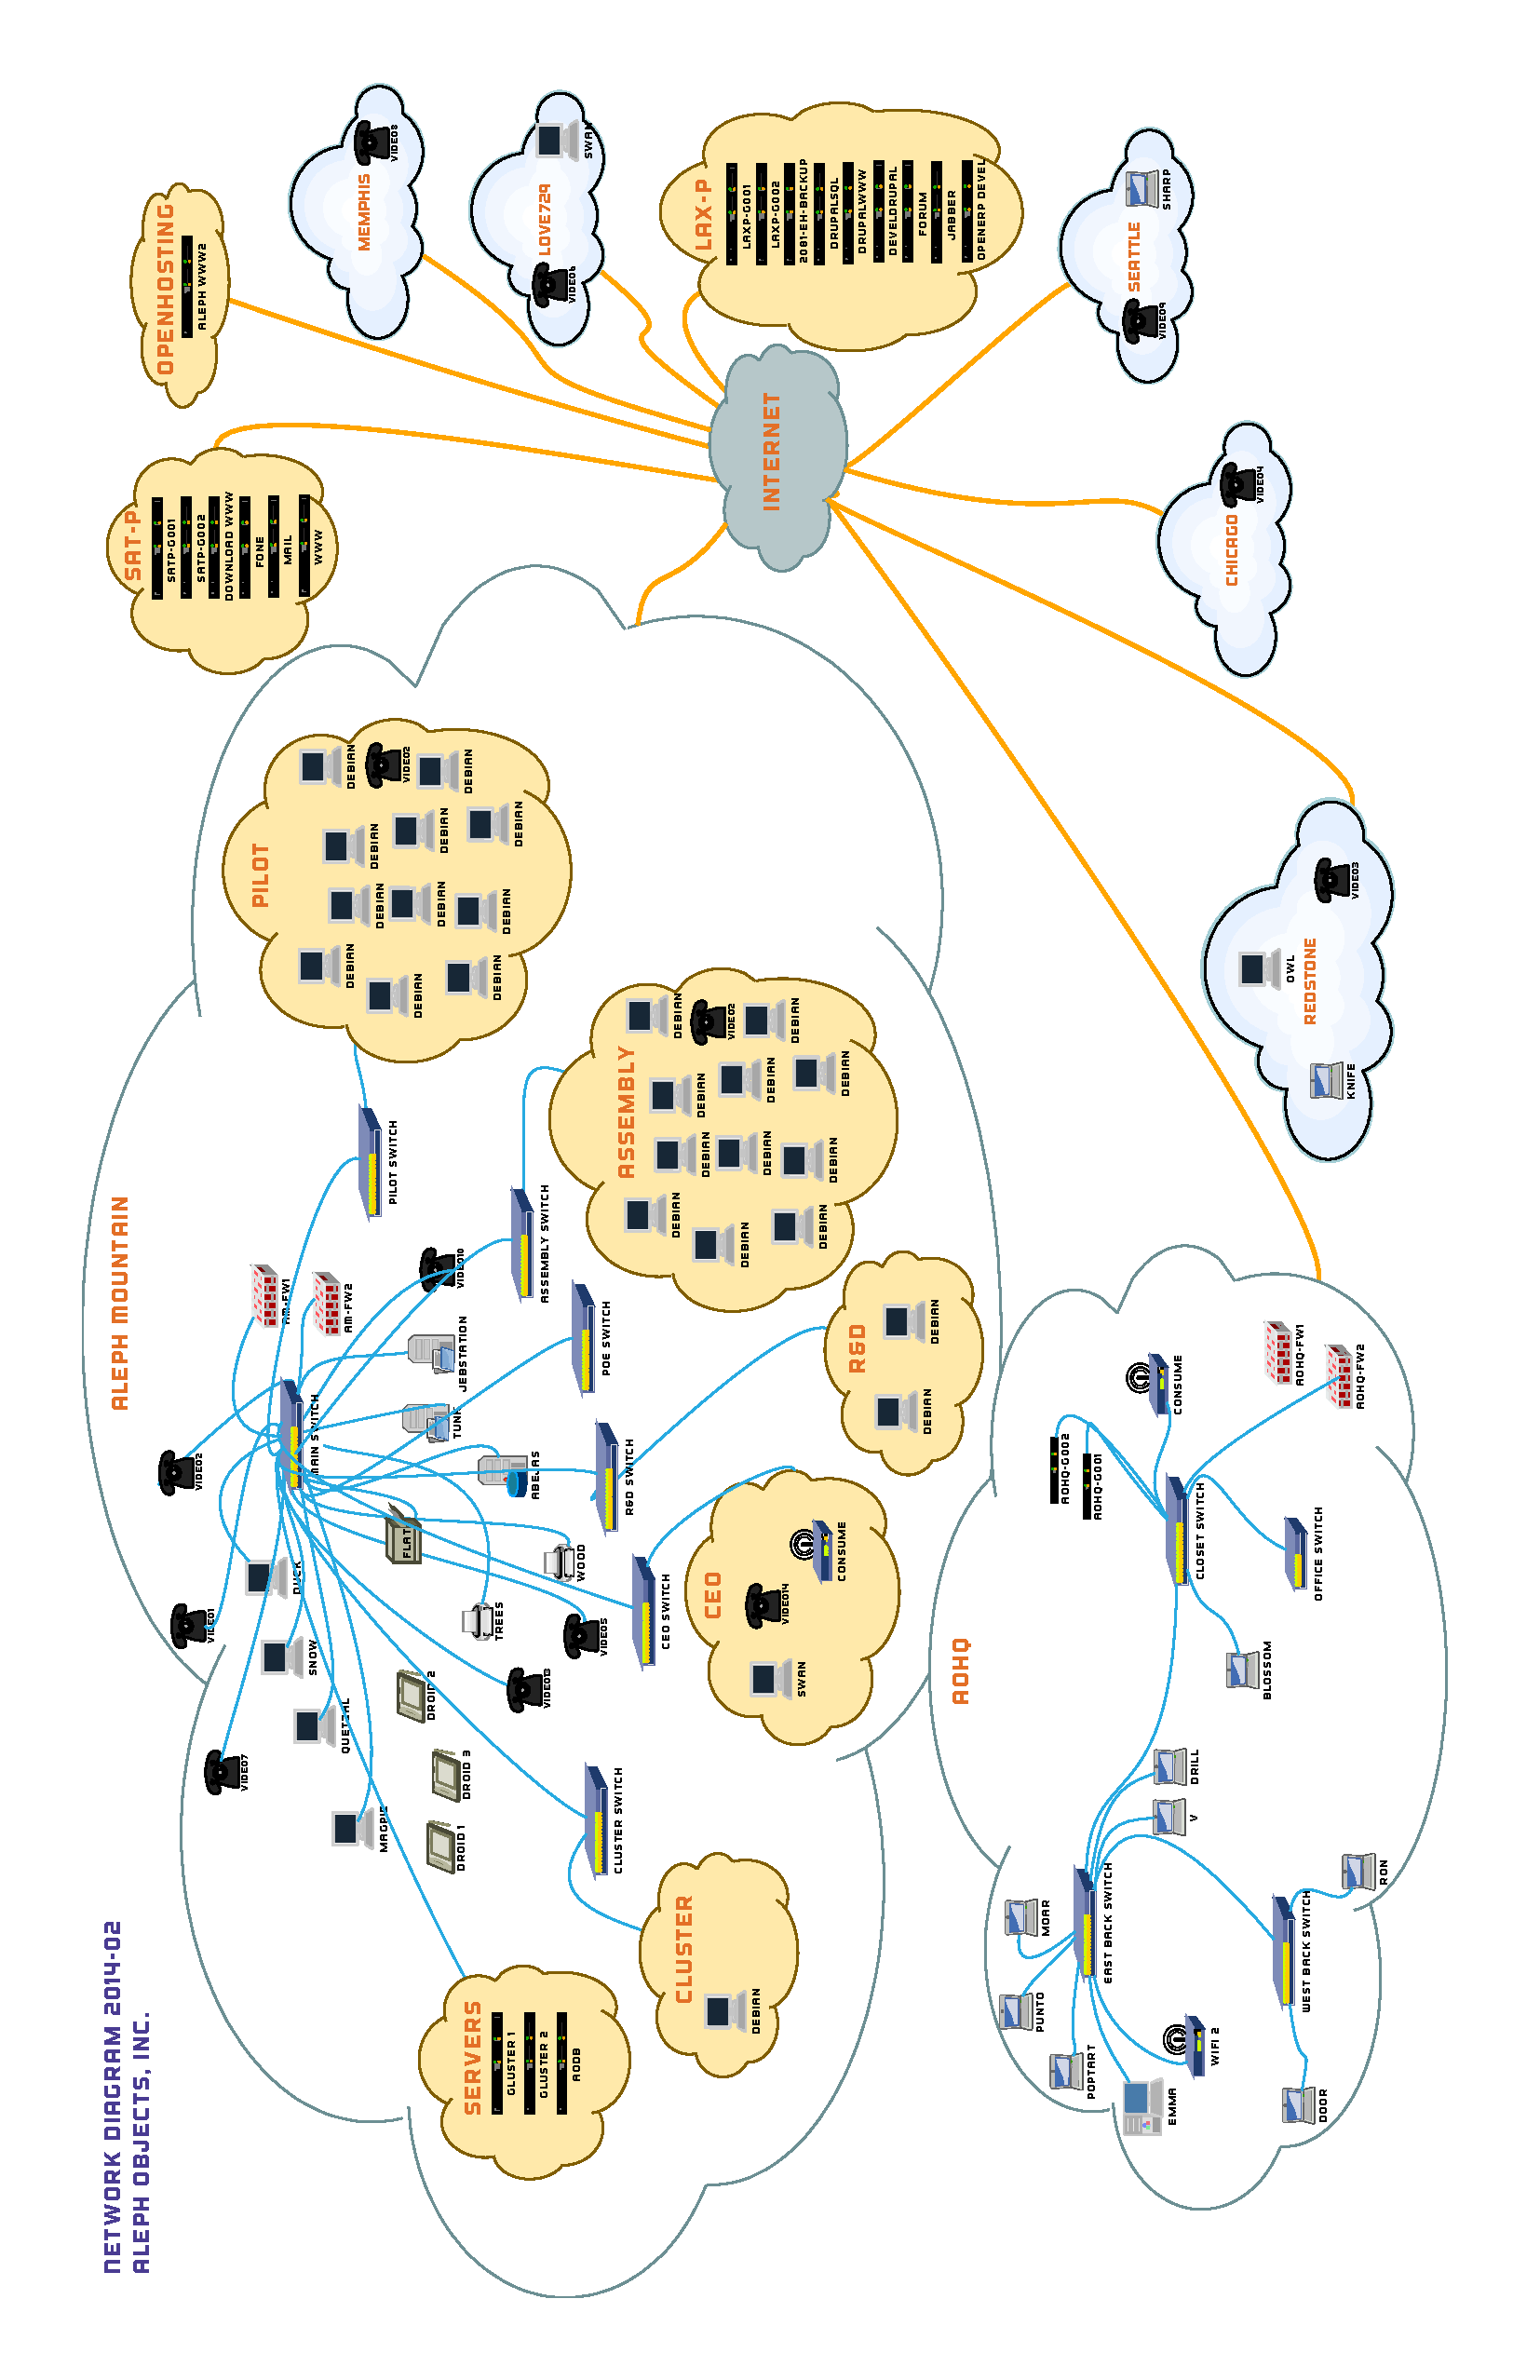
\includegraphics[keepaspectratio=true,height=1.10\textheight,width=1.00\textwidth,angle=-90]{ao-network.pdf}
 \caption{Network Diagram}
 \label{fig:ao_net_dia}
\end{sidewaysfigure}

\begin{sidewaysfigure}[p]
\thisfloatpagestyle{empty}
% The ao-network-overview.pdf built in calligraflow.
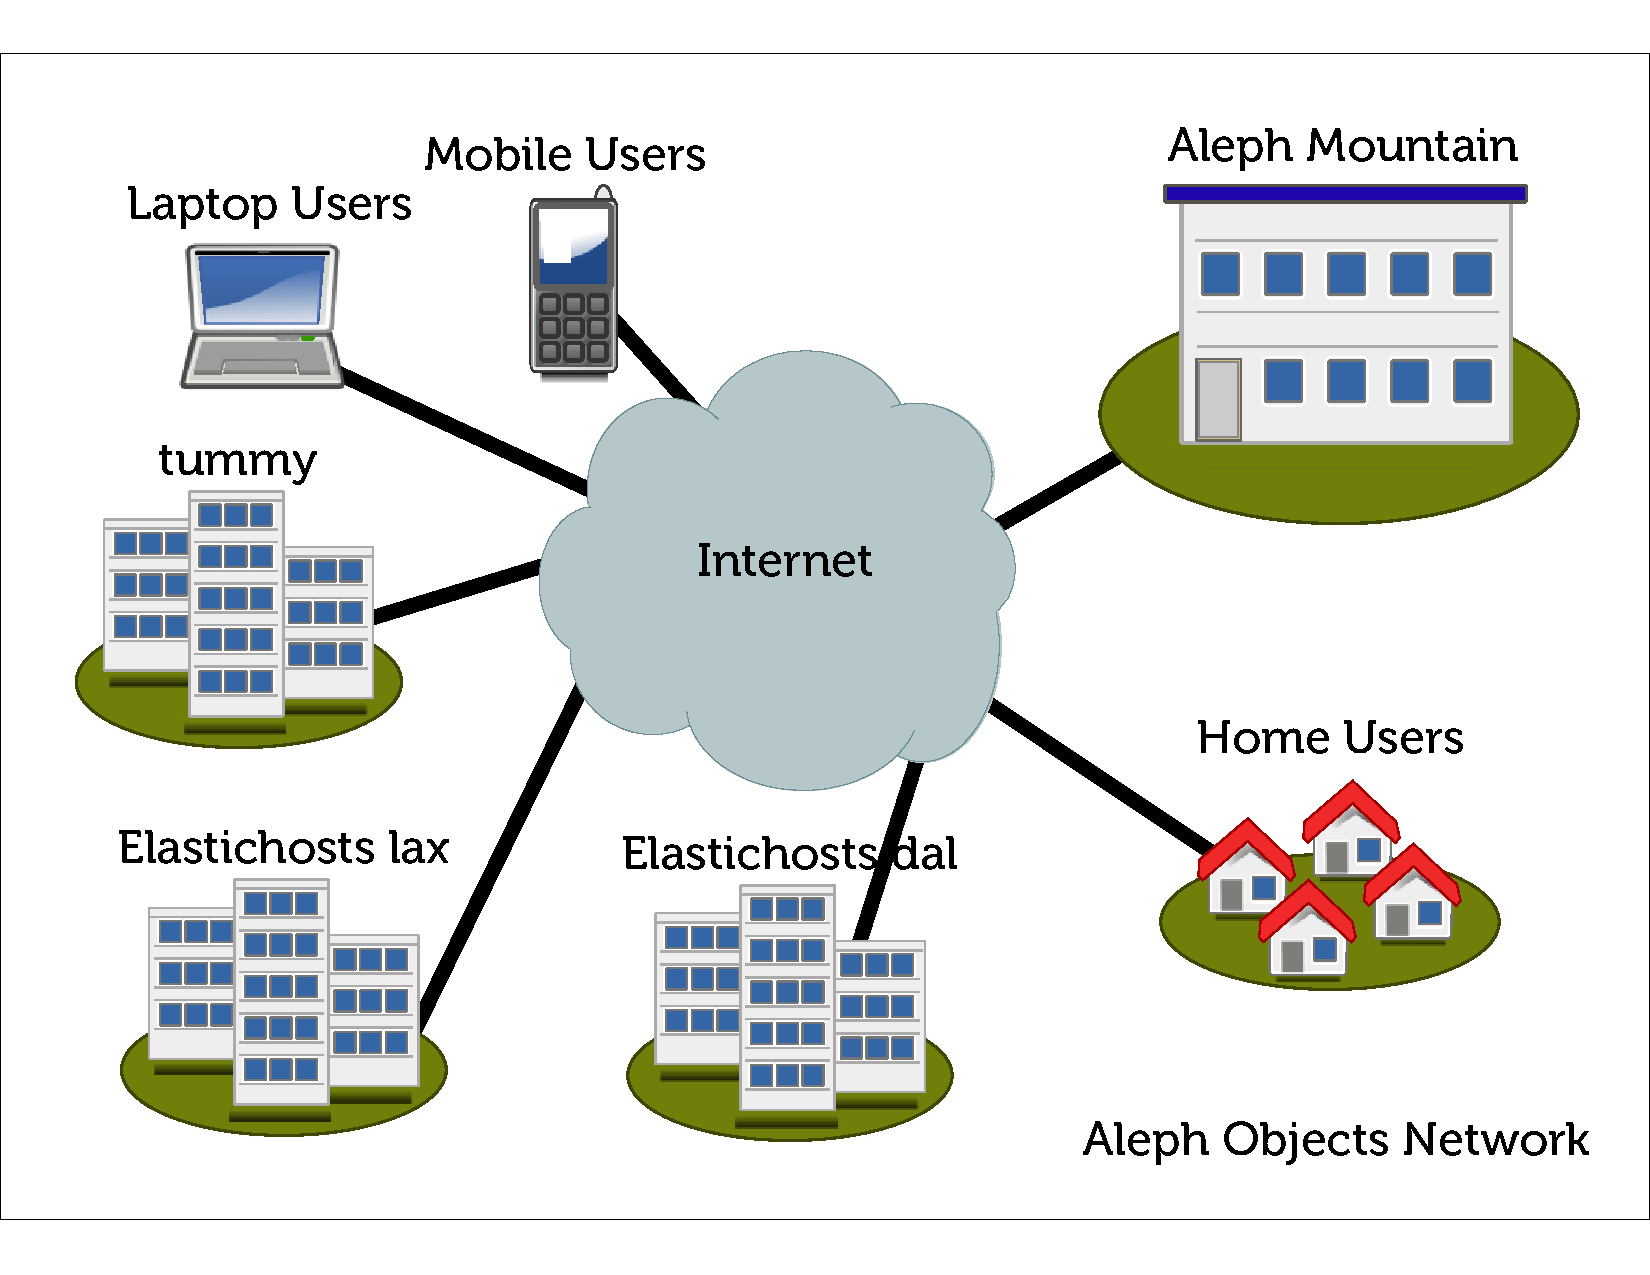
\includegraphics[keepaspectratio=true,height=1.10\textheight,width=1.00\textwidth,angle=0]{ao-network-overview.pdf}
 \caption{Aleph Objects Network Overview}
 \label{fig:ao_net_overview}
\end{sidewaysfigure}

